%
% $Id: $
%
%
% Compilar a .pdf con LaTeX (pdflatex)
% Es necesario instalar Beamer (paquete latex-beamer en Debian)
%

%
% Gráficos:
% Los gráficos pueden suministrarse en PNG, JPG, TIF, PDF, MPS
% Los EPS deben convertirse a PDF (usar epstopdf)
%

\documentclass[17pt,aspectratio=169]{beamer}
\usetheme[orchid]{Hannover}
%\usebackgroundtemplate{
\includegraphics[width=\paperwidth]{format/libresoft-bg-soft.png}}
\usepackage[spanish]{babel}
\usepackage[utf8]{inputenc}
\usepackage{graphics}
\usepackage{amssymb} % Simbolos matematicos

%\definecolor{libresoftgreen}{RGB}{162,190,43}
%\definecolor{libresoftblue}{RGB}{0,98,143}

%\setbeamercolor{titlelike}{bg=libresoftgreen}

%% Metadatos del PDF.
%% \hypersetup{
%%   pdftitle={La tecnología no es neutra},
%%   pdfauthor={Jesús M. González Barahona},
%%   pdfcreator={GSyC/LibreSoft, Universidad Rey Juan Carlos},
%%   pdfproducer=PDFLaTeX,
%%   pdfsubject={},
%% }
%%

\newcommand\YUGE{\fontsize{48}{60}\selectfont}

\AtBeginSection[]
{
  {
    \usebackgroundtemplate{\includegraphics[width=\paperwidth,height=\paperheight]{\secimage}}
    \begin{frame}<beamer>

      \begin{center}
        {\YUGE\bf\insertsection}
      \end{center}
    \end{frame}
  }
  \renewcommand{\secimage}{figs/bookpages}
}

% Pixbay
% NikolayFrolochkin
% https://pixabay.com/en/book-reading-library-literature-1261800/
% License: CC0 Creative Commons
\newcommand{\secimage}{figs/bookpages}

\begin{document}

\title{Publicación abierta en TIC}
%\subtitle{}
\author{Jesús M. González Barahona}
\institute{Correo: jgb@gsyc.es ~~~~ Twitter: @jgbarah2 \\
  Universidad Rey Juan Carlos \\ }

\date{Programa de Doctorado en TIC \\
  Universidad Rey Juan Carlos \\
  Móstoles, 7 de junio de 2019\\
{\small \url{https://jgbarah.github.io/presentations}} \\}

\frame{
\maketitle
}
%% \begin{center}
%% 
\includegraphics[width=6cm]{format/gsyc-urjc}
%% \end{center}

%% \begin{frame}

%%   {\Large
%%     \tableofcontents
%%   }

%% \end{frame}

%%---------------------------------------------------------------
%%---------------------------------------------------------------
\section{Motivación}

%%---------------------------------------------------------------
\begin{frame}

  {\em \Large
    Por primera vez \\
    tenemos herramientas \\
    que nos permiten acceder, \\
    de forma simple, rápida y barata, \\
    a todo el conocimiento \\
    científico producido por la humanidad...\\
  }
  
\end{frame}

%%---------------------------------------------------------------
\begin{frame}

  {\em \Large
    ...y lo estamos impidiendo \\
    con un modelo económico y legal \\
    de la era de la información en papel \\
  }
  
\end{frame}

%%---------------------------------------------------------------
%%---------------------------------------------------------------
\section{Definiciones}

%%---------------------------------------------------------------

\begin{frame}
\frametitle{BOAI}

Budapest Open Access Initiative, 2002

\vspace{.5cm}

\begin{quote}
  ``world-wide electronic distribution of the peer-reviewed journal literature and completely free and unrestricted access''
\end{quote}

\begin{flushright}
  {\small \url{https://budapestopenaccessinitiative.org}}
\end{flushright}

\end{frame}

%%---------------------------------------------------------------

\begin{frame}
\frametitle{BDoOA}

Berlin Declaration on Open Access, 2003

\vspace{.3cm}

\begin{quote}
  ``El (los) autor(es) [...] deben garantizar el derecho gratuito, irrevocable y mundial de acceder a el trabajo, lo mismo que licencia para copiarlo, usarlo, distribuirlo, transmitirlo y exhibirlo públicamente, y para hacer y distribuir trabajos derivados [...]"
\end{quote}


\begin{flushright}
  {\small \url{https://openaccess.mpg.de/Berlin-Declaration}}
\end{flushright}

\end{frame}

%%---------------------------------------------------------------

\begin{frame}
\frametitle{Condiciones}

\begin{itemize}
\item Derecho de acceso (consulta)
\item Derecho de copia
\item Derecho de trabajos derivados
\item Obra y materiales en formatos electrónicos ``adecuados''
\item Depósito de la obra y materiales complementarios \\
  en un archivo abierto
\end{itemize}

Todo, con atribución de autoría

\end{frame}

%%---------------------------------------------------------------

\begin{frame}
\frametitle{Materiales cubiertos}

\begin{itemize}
\item resultados de investigación (artículos)
\item datos crudos y metadatos
\item materiales fuente (notas)
\item representaciones digitales (gráficos, multimedia)
\item programas de ordenador
\end{itemize}

\end{frame}

%%---------------------------------------------------------------

\begin{frame}
\frametitle{Archivo abierto}

\begin{itemize}
\item Estándares de acceso adecuados \\
  (ejemplo: Open Archive Definitions)
\item mantenido por una organización ``fiable''
\item vocación de distribucion universal, \\
  interoperabilidad, \\
  archivo a largo plazo
\end{itemize}

\end{frame}

%%---------------------------------------------------------------
%%---------------------------------------------------------------
\section{Tipos de acceso abierto}

%%---------------------------------------------------------------
\begin{frame}

\begin{itemize}
\item Gold
\item Green
\item Hybrid
\item Bronze
\item Diamond/platinum
\item Black
\end{itemize}

\end{frame}

%%---------------------------------------------------------------
\begin{frame}
\frametitle{Gold open access}

\begin{itemize}
\item Publicaciones
\item con todo el contenido disponible gratuitamente
\item de forma inmediata
\item con licencia de reutilización
\end{itemize}

Ejemplos: PlosOne, PeerJ

\begin{flushright}
  \url{https://journals.plos.org/plosone/} \\
  \url{https://peerj.com/} \\
\end{flushright}
\end{frame}

%%---------------------------------------------------------------
\begin{frame}
\frametitle{Green open access}

\begin{itemize}
\item Autoarchivo por los autores
\item Idealmente: postprint
\item En muchos casos: sólo preprint (yellow/blue)
\item Ver la clasificación Sherpa/Romeo
\end{itemize}

\vspace{.5cm}

Preprint: antes de revisión \\
Postprint: después de revisión (versión del autor) \\
\end{frame}

%%---------------------------------------------------------------
\begin{frame}
\frametitle{Hybrid open access}

\begin{itemize}
\item Publicaciones
\item con mezcla de articulos cerrados y abiertos
\item parte de los ingresos vienen de subscripciones
\end{itemize}

\begin{flushright}
  Ejemplo: Springer Open Choice \\
  {\small \url{https://www.springer.com/gp/open-access/springer-open-choice}} \\
\end{flushright}
\end{frame}

%%---------------------------------------------------------------
\begin{frame}
\frametitle{Bronze open access}

\begin{itemize}
\item Publicaciones
\item artículos comienzan cerrados
\item acceso abierto tras periodo de embargo
\end{itemize}

A veces se refiere a permiso de lectura, pero sin licencia

\end{frame}

%%---------------------------------------------------------------
\begin{frame}
\frametitle{Diamond/platinum OA}

\begin{itemize}
\item Publicaciones gold open access
\item que no cobran a los autores
\end{itemize}

\begin{flushright}
  Fair Open Access Principles \\
  {\small \url{https://fairopenaccess.org/the-fair-open-access-principles/}} \\
  Free Journal Network \\
  {\small \url{https://freejournals.org}} \\
\end{flushright}
\end{frame}

%%---------------------------------------------------------------
\begin{frame}
\frametitle{Conceptos relacionados}

\begin{itemize}
\item Preprints
\item Autoarchivo
\item DOI
\item ORCID
\item Índices accesibles: Scholar, DBLP, Dialnet
\end{itemize}

\end{frame}


%%---------------------------------------------------------------
%%---------------------------------------------------------------
\section{Recursos}

%%---------------------------------------------------------------
\begin{frame}

  \begin{itemize}
  \item ``Open access'' en Wikipedia \\
    {\small \url{https://en.wikipedia.org/wiki/Open_access}}
  \item Directory of Open Access Journals \\
    {\small \url{https://www.doaj.org}}
  \item EU Comission policy on open science \\
    {\small \url{https://ec.europa.eu/research/openscience/}}
  \end{itemize}

\end{frame}

%%---------------------------------------------------------------
\begin{frame}
\frametitle{Sherpa/Romeo}

\begin{center}
  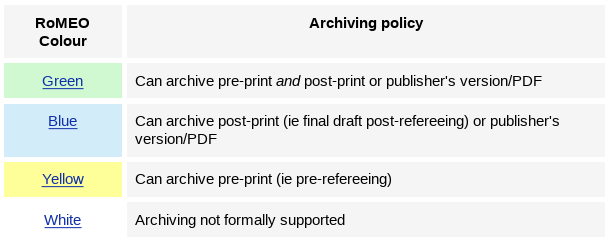
\includegraphics[width=12.5cm]{figs/sherpa-romeo}
\end{center}  

\begin{flushright}
{\small \url{http://sherpa.ac.uk/romeo/index.php}}
\end{flushright}

\end{frame}

%%---------------------------------------------------------------
\begin{frame}
\frametitle{Arxiv}

\begin{center}
  
\includegraphics[width=12.5cm]{figs/arxiv}
\end{center}  

\begin{flushright}
{\small \url{https://arxiv.org}}
\end{flushright}

\end{frame}

%%---------------------------------------------------------------
\begin{frame}
\frametitle{Zenodo}

\begin{center}
  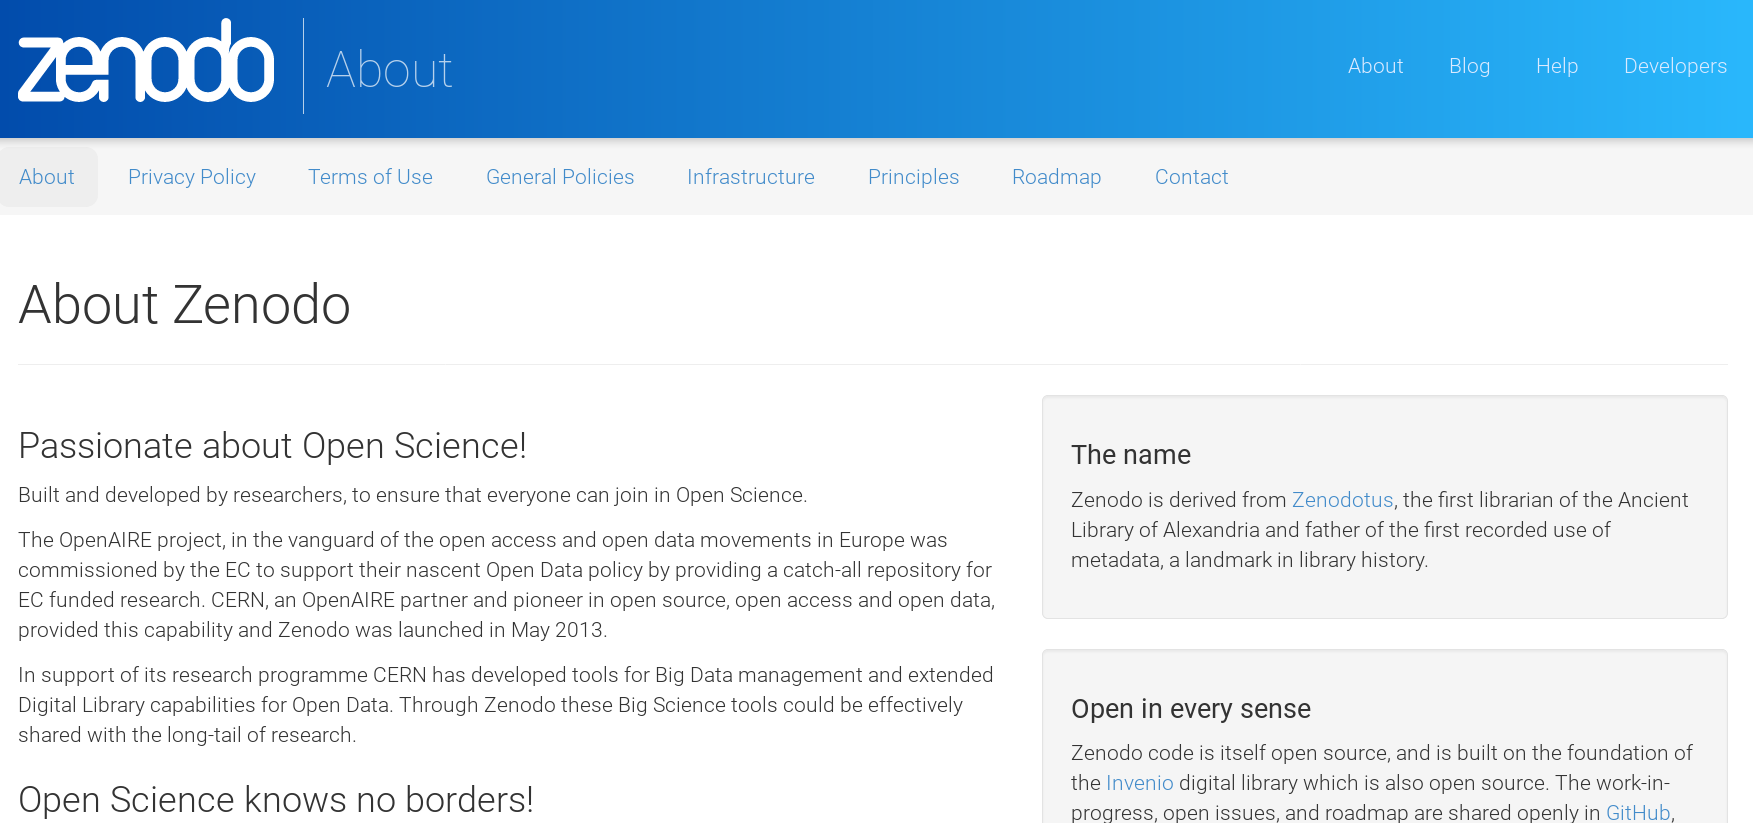
\includegraphics[height=5.5cm]{figs/zenodo}
\end{center}  

\begin{flushright}
{\small \url{https://zenodo.org}}
\end{flushright}

\end{frame}

%%---------------------------------------------------------------
%%---------------------------------------------------------------
\section{Ejemplos en TIC}

%%---------------------------------------------------------------
\begin{frame}
\frametitle{IEEE (2019)}

\begin{itemize}
\item ~1.750 USD por articulo
\item Se permite green open access \\
  (post-review preprints) \\
\end{itemize}

\begin{flushright}
{\footnotesize \url{http://www.ieee.org/publications_standards/publications/authors/open_access.html}}
\end{flushright}

\end{frame}

%%---------------------------------------------------------------
\begin{frame}
\frametitle{IEEE (2019)}

\begin{itemize}
\item ~1.700 USD por articulo
\item Se permite green open access \\
  (post-review preprints) \\
\end{itemize}

\begin{flushright}
{\footnotesize \url{https://www.acm.org/open-access}}
\end{flushright}

\end{frame}

%%---------------------------------------------------------------
\begin{frame}
\frametitle{Elsevier (2019)}

\begin{itemize}
\item Opciones gold e hybrid
\item ~150 - ~5.000 USD por artículo
\item Se permite green open access \\
  (pre-prints) \\
  (post-prints, tras periodo de embargo) \\
\end{itemize}

\begin{flushright}
{\footnotesize \url{https://www.elsevier.com/about/open-science/open-access}}
\end{flushright}

\end{frame}

%%---------------------------------------------------------------
\begin{frame}
\frametitle{Springer (2019)}

\begin{itemize}
\item Opciones gold e hybrid
\item ~2,200 EUR por artículo
\item Se permite bronze open access \\
  (post-prints, tras periodo de embargo, 1 año) \\
\end{itemize}

\begin{flushright}
{\footnotesize \url{http://www.springer.com/gp/open-access}}
\end{flushright}

\end{frame}


%%---------------------------------------------------------------
%%---------------------------------------------------------------
\section{Temas relacionados}

%%---------------------------------------------------------------
\begin{frame}
\frametitle{Open Science}

Hacer la investigación científica y sus resultados accesibles a todos los niveles de la sociedad

\begin{itemize}
\item publicaciones
\item datos
\item muestras física
\item software
\end{itemize}

\end{frame}

%%---------------------------------------------------------------
\begin{frame}
\frametitle{Open Data}

{\em ``Datos que cualquiera puede usar, modificar \\
  y compartir para cualquier propósito'' \\
}
\begin{flushright}
  \url{http://opendefinition.org/}
\end{flushright}

{\em ``Datos libremente disponibles para \\
cualquiera, que se pueden utilizar y \\
republicar, sin restricciones de patentes, \\
derechos de autor, ni de otro tipo.'' \\
}

\begin{flushright}
  \url{https://en.wikipedia.org/wiki/Open_data}
\end{flushright}

\end{frame}

%%---------------------------------------------------------------
%%---------------------------------------------------------------
\section{URJC}

%%---------------------------------------------------------------
\begin{frame}
\frametitle{OfiLibre}

Oficina de Conocimiento y Cultura Libres:

\begin{itemize}
\item Publicación abierta, datos abiertos, \\
  cultura libre, software libre
\item Coordinación, formación, visibilización \\
  apoyo, fomento
\end{itemize}

\begin{flushright}
  \url{https://urjc.es/ofilibre}
\end{flushright}

\end{frame}

%%---------------------------------------------------------------
% LICENCIA DE REDISTRIBUCION DE LAS TRANSPAS
\frame{
~
\vspace{3cm}

\begin{flushright}
{\small
\copyright 2019 Jesús M. González Barahona. \\

  Algunos derechos reservados. \\
  Este artículo se distribuye bajo la licencia \\
  ``Reconocimiento-CompartirIgual 3.0 España'' \\
  de Creative Commons, \\
  disponible en \\
}
{\footnotesize
  \url{https://creativecommons.org/licenses/by-sa/3.0/es/} \\
}
\end{flushright}
}

\end{document}
